 
\begin{center}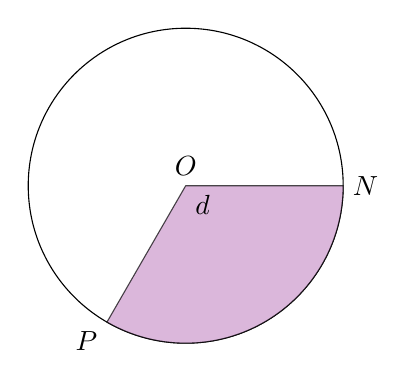
\begin{tikzpicture}
\draw(0,0)node[anchor=south]{$O$}circle(2);
\fill[draw=black,fill=blue!20!pink,opacity=0.7](0,0)--(2,0)arc(0:-120:2)--(0,0);
\draw(2,0)node[anchor=west]{$N$}(-120:2)node[anchor=north east]{$P$};
\draw(0,0)node[anchor=north west]{$d\degree$};
\end{tikzpicture}\\
Note: Figure not drawn to scale.
\end{center}
In the figure above, the circle has center $O$ and has radius $7$.  If the sector bounded by the arc $\wideparen{NP}$ and radii $\overline{OP}$ and $\overline{NO}$ has an area between $44$ and $45$, what is one possible \underline{integer} value for $d$?
\\\\


\ifsat
	\begin{enumerate}[label=\Alph*)]
	\end{enumerate}
\else
\fi

\ifacteven
	\begin{enumerate}[label=\textbf{\Alph*.},itemsep=\fill,align=left]
		\setcounter{enumii}{5}
		\item None of these. 
	\end{enumerate}
\else
\fi

\ifactodd
	\begin{enumerate}[label=\textbf{\Alph*.},itemsep=\fill,align=left]
		\item None of these. 
	\end{enumerate}
\else
\fi

\ifgridin
$103$ or $104$ or $105$
\else
\fi

